\documentclass[10pt,conference,letterpaper]{IEEEtran}
\IEEEoverridecommandlockouts
% The preceding line is only needed to identify funding in the first footnote. If that is unneeded, please comment it out.
\usepackage{cite}
\usepackage{amsmath,amssymb,amsfonts}
\usepackage{algorithmic}
\usepackage{graphicx}
\usepackage{textcomp}
\usepackage{xcolor}
\usepackage{booktabs}
\usepackage{bbding}
\usepackage{stfloats}
\usepackage{makecell}
%\usepackage{algorithm}
%\usepackage{algorithmicx}
\def\BibTeX{{\rm B\kern-.05em{\sc i\kern-.025em b}\kern-.08em
T\kern-.1667em\lower.7ex\hbox{E}\kern-.125emX}}
\begin{document}

    \title{Analysis of the Design of Several Modern Programming Languages\\
%    {\footnotesize \textsuperscript{*}
%    Note: Sub-titles are not captured in Xplore andshould not be used
%    }
%    \thanks{Identify applicable funding agency here. If none, delete this.}
    }

    \author{\IEEEauthorblockN{Xudong Wang, Zhimei Zhang}
    \IEEEauthorblockA{\textit{College of Computer Science \& Technology} \\
    \textit{Qingdao University}\\
    Qingdao, China}
%    \and
%    \IEEEauthorblockN{2\textsuperscript{nd} Given Name Surname}
%    \IEEEauthorblockN{}
%    \IEEEauthorblockA{\textit{dept. name of organization (of Aff.)} \\
%    \textit{name of organization (of Aff.)}\\
%    City, Country \\
%    email address or ORCID}
    }

    \maketitle

    \begin{abstract}
        Modern programming languages are analyzed in terms of design through several aspects of programming language theory - programming paradigm, type system, and performance. The programming paradigm section gives a method for evaluating the degree of programming paradigm support and uses this method to evaluate the degree of programming paradigm support in modern programming languages. Thus, the connection between programming paradigms and application scenarios is obtained. The type system section analyzes the commonalities of the type systems of modern programming languages. The performance section quantitatively analyzes the performance of modern programming languages by means of benchmarking, and qualitatively analyzes the connection between the performance of programming languages and application scenarios. Finally, it is concluded that the design and practice of programming languages evolve dynamically, and the design of programming languages is closely related to their application scenarios.
    \end{abstract}

    \begin{IEEEkeywords}
        modern programming language,
        programming language design,
        programming language,
        programming paradigm,
        type system,
        benchmarking.
    \end{IEEEkeywords}


    \section{Introduction}

%In programming language theory(PLT), programming language design has always been an important topic. Because programming language design integrates various branches of PLT, it is the prerequisite for the final realization of programming language. By analyzing the design of modern programming languages(MPL), we can obtain the trend of programming language development, i.e., the programming language design can be fed back from the application point of view.
%
%By and large, the overall amount of literature on the analysis of
%programming language design is relatively small.
%M Coblenz argues that programming language design should be
%considered in terms of several theories related to programming
%languages and gives a way of evaluating programming language
%design\cite{coblenz2018interdisciplinary}.
%A Stefika gives some issues to consider in programming language
%design and argues that type systems are crucial for
%programming languages\cite{stefik2014programming}.
%However, the above results focus on a qualitative analysis of
%programming language design and lack some concrete examples.
%LA Meyerovich analyzes the usage of popular programming languages
%to give best practices in programming language design
%through statistics\cite{meyerovich2013empirical}.
%This analytical approach is somewhat lacking in theoretical and
%systematic aspects.
%F Morandat provides a systematic analysis of the R language,
%including performance, syntactic design, and application
%scenarios\cite{morandat2012evaluating}.
%The article adopts a better research approach and can be used to
%broaden the analysis perspective based on that article.
%Currently, there is a lack of a systematic, theoretical and
%practical, wide-ranging, application-oriented analysis of
%programming language design.
%
%By analyzing the design of MPL, this paper draws the influence of different programming language factors on the application. e.g., as programming languages evolve, why does the level of paradigm support in MPLs keep changing, what type systems are in MPLs, how MPLs keep programs efficient, and so on.

%%%%%%%%%%%%%%%%%%%%%%%%%
%In programming language theory (PLT), programming language
%design has always been an important topic.
%The design of a programming language would influence the way programmers think.
%Alan J. Perlis has said, “A language that doesn't affect the
%way you think about programming, is not worth knowing.”\cite{perlis1982special}
%
%
%However, the overall amount of literature on the analysis of
%programming language design is relatively small.
%M. Coblenz et.al argues that programming language design should be considered in terms
%of several related theories and proposes a way of evaluating programming
%language design\cite{coblenz2018interdisciplinary}.
%A. Stefika and S. Hanenberg give some issues to consider when designing
%a programming language and argues that type systems are crucial for
%programming languages\cite{stefik2014programming}.
%However, the above papers focus on qualitative analysis and lack
%some concrete examples.
%L. A. Meyerovich and A. S. Rabkin analyze the popularity of commonly
%used programming languages through statistics, which is relatively
%flawed in theoretical and systematic aspects\cite{meyerovich2013empirical}.
%F. Morandat et.al provides a systematic analysis of the R language,
%including performance, syntactic design, and application scenarios\cite{morandat2012evaluating}.
%The paper applies a relatively good method, but it analyzes only one language.
%
%
%In this paper, by analyzing the design of certain modern programming
%languages (MPLs) we chose, we conduct a systematic, theoretical and practical,
%and application-oriented analysis of the design of multiple programming languages.
%The trend of programming language development is obtained, and some design
%details are explained and discussed.
%Specifically, why the paradigm of MPLs keeps changing, what kind of
%type systems MPLs use, and how MPLs keep programs efficient.
%
%The paper is organized as following.
%Section 2 describes the features of MPLs and the criteria
%to evaluate the design of programming languages.
%Section 3 presents the analysis of paradigms of multiple MPLs we select in detail.
%Section 4 shows the results of type systems of the selected MPLs.
%Section 5 evaluate the performance of the selected MPLs.
%In Section 6, we give the conclusion.
%%%%%%%%%%%%%%%%%%%%%%%%%

In programming language theory (PLT), programming language
design has always been an important topic.
The design of a programming language would influence the way programmers think.
Alan J. Perlis has said, “A language that doesn’t affect the
way you think about programming, is not worth knowing.”\cite{perlis1982special}

However, the overall amount of literature on the analysis of
programming language design is relatively small.
M. Coblenz et.al argues that programming language design should be considered in terms
of several related theories and proposes a way of evaluating programming
language design\cite{coblenz2018interdisciplinary}.
A. Stefika and S. Hanenberg give some issues to consider when designing
a programming language and points out that type systems are crucial for
programming languages\cite{stefik2014programming}.
However, the above papers focus on qualitative analysis and lack
some concrete examples.
L. A. Meyerovich and A. S. Rabkin analyze the popularity of commonly
used programming languages through statistical counting,
which is relatively flawed in theoretical and systematic aspects\cite{meyerovich2013empirical}.
F. Morandat et.al provides a systematic analysis of the R language,
including performance, syntactic design, and application scenarios\cite{morandat2012evaluating}.
The paper applies a relatively good method, but it analyzes only one language.

%In this paper, we conduct a systematic, theoretical and practical,
%and application-oriented analysis of the design of multiple programming
%languages (MPLs).
%By analyzing the design of certain MPLs we chose, the trend of programming
%language development is obtained,
%and some design details are explained and discussed.
%Specifically, why the paradigm of MPLs keeps changing,
%what kind of type systems MPLs use, and how MPLs keep programs efficient.
In this paper, we conduct a systematic analysis of the design of
multiple modern programming languages (MPLs).
Our contribution is that, by analyzing programming paradigms, type systems, and performance of these languages' design,
we obtain their development trend to enable users to select suitable languages according to the application scene.


%The paper is organized as follows.
%Section 2 describes the features of MPLs and the criteria to evaluate the design of programming languages.
%Section 3 presents the analysis of paradigms of multiple MPLs we select in detail.
%Section 4 shows the results of type systems of the selected MPLs.
%Section 5 evaluates the performance of the selected MPLs.
%In Section 6, we give the conclusion.


    \section{Selecting several modern programming languages}

%We give the definition for MPL, accordingly choose nine MPLs,
%and explain the aspects of their designs to be analyzed.


%There is no uniform definition for MPL\@.
%Many researchers define it in different ways, such as finding
%connections between software engineering\cite{ModernProgrammingLanguagesSoftwareEnginerring}
%and the development of MPLs or elaborating
%around abstractions\cite{ModernProgrammingLanguagesAbstraction}.
%The above are correct in their respective fields,
%and here the definition is abstracted and extended to
%adapt to more domains.
%By studying the intersection of different definitions,
%a more general definition of MPLs derives.
%It is an obvious fact, that as the practice of
%programming languages continues to deepen, so does
%the definition of MPL. This is because PLT is a field
%where practice and theory go hand in hand.
%Although its definition is constantly changing, some
%core elements remain the same.
%Here are a few features of MPLs.

%\subsection{The features of modern programming language}

Researchers define MPL in different ways.
For example, some scholars define it from the perspective of software
engineering – as it develops, programming languages evolve into MPLs\cite{ModernProgrammingLanguagesSoftwareEnginerring}.
While others consider the key feature of MPL its abstraction\cite{ModernProgrammingLanguagesAbstraction}.
%In fact, as the practical technology of programming languages progresses,
%the definition of MPL will keep altering, because it is a combination
%of both theory and practice.
%However,although its definition keeps altering,
%some core contents remain unchanged.
%After studying multiple definitions given in the literature, we present a
%more general description for MPL, which has the following features:

%\begin{enumerate}
%    \item Substance over form. It should provide descriptive grammatical structures, rather than hand-in-hand telling the machine what to do. This item emphasizes the abstraction of machine functions.
%    \item Semantic consistency. For similar grammatical structures, there should be similar grammatical functions.
%    \item Syntax bootstrapping. For non-core grammatical features, based on following semantic consistency, they should be composed of core grammatical features.
%    \item Paradigm convergence. Multiple programming paradigms should be provided without forcing users to use a particular programming paradigm.
%\end{enumerate}

%\begin{enumerate}
%    \item Substance over form. MPLs should emphasize what is important to the users and restrain what is not.
%    \item Semantic consistency. For similar grammatical structures, there should be similar semantics.
%    \item Syntax bootstrapping. For non-core grammars, following semantic consistency, they should be composed of core grammars.
%    \item Paradigm convergence. Multiple programming paradigms should be provided without forcing users to use a particular one.
%\end{enumerate}

%\begin{table*}[hb]
%    \caption{Features that a well-designed programming language should have}
%    \label{tab:evaluate}
%    \begin{center}
%        \begin{tabular}{ccc}
%            \toprule
%            Evaluation Item & Meaning & Related Content \\
%            \midrule
%            Expressiveness &
%            \makecell[l]{
%                For abstract and complex business logic, programming \\
%                languages can provide a concise way to describe it.
%            }
%            & Programming Paradigm, Type System \\
%            \midrule
%            Maintainability &
%            \makecell[l]{
%                After completing the business logic according to \\
%                standard coding specifications, it is also easy to add new \\ features or
%                fix bugs subsequently.
%            }
%            & Programming Paradigm, Type System \\
%            \midrule
%            Reliability &
%            \makecell[l]{
%                Non-crash under extreme conditions after completing \\
%                business logic according to standard coding specifications.
%            }
%            & Programming Paradigm, Type System \\
%            \midrule
%            Performance &
%            \makecell[l]{
%                Deploying a software system written in this programming \\
%                language takes up fewer hardware resources when running \\ on the target
%                machine.
%            }
%            & Time Overhead, Memory Overhead \\
%            \bottomrule
%        \end{tabular}
%    \end{center}
%\end{table*}

%\subsection{Selecting modern programming languages to be analyzed}

%We select the MPLs to be analyzed based on the following considerations.
%We first select the current most popular programming languages.
%Next, there are many classification standards for programming languages.
%For each standard, the selected programming languages should cover most of the categories.
%Finally, we should focus on the new programming languages.
%These programming languages have absorbed the advantages of past languages and
%alleviated their inherent shortcomings.

According to the data of the IEEE spectrum,the top five popular programming
languages in 2021 are Python, Java, C, C ++, and JavaScript\cite{IEEETopProgrammingLanguages}.
Among them, C cannot be considered an MPL, due to its underlying syntax design.
We thus select the other four popular programming languages as our research objects.
According to the degree of popularity, we select five new-born MPLs -
Go, Swift, Dart, Rust, and Kotlin (where Swift and Dart are equally popular).
Coincidentally, these languages were also released in this order.
%It should be noted that, even though nowadays they are not exactly in line with the
%features of MPL, they were the representative symbols of MPLs back when they
%were initially developed.

%For the selection of programming language, the first thing is to pay attention to the most popular trend at the moment, so the selected programming language must cover the most commonly used. Secondly, there are many classification standards for programming languages. For each division standard, the selected programming language should cover most of the options. Then, it should focus on highlighting the new programming language with excellent design in recent years. These programming languages have absorbed the advantages of past programming languages and improved their inherent shortcomings. From these selected MPLs, we can see the development trend of application-oriented programming languages over the years.


%In addition, they all have similar type systems and support AOT compilation,
%and although not all of them use garbage collection memory management,
%they all move away from manual memory management.
%These are all common features of MPLs in today’s application environment.


%The timeline of the birth of the nine selected MPLs is shown in Figure~\ref{fig:timeline}.
%
%\begin{figure}[htbp]
%    \centerline{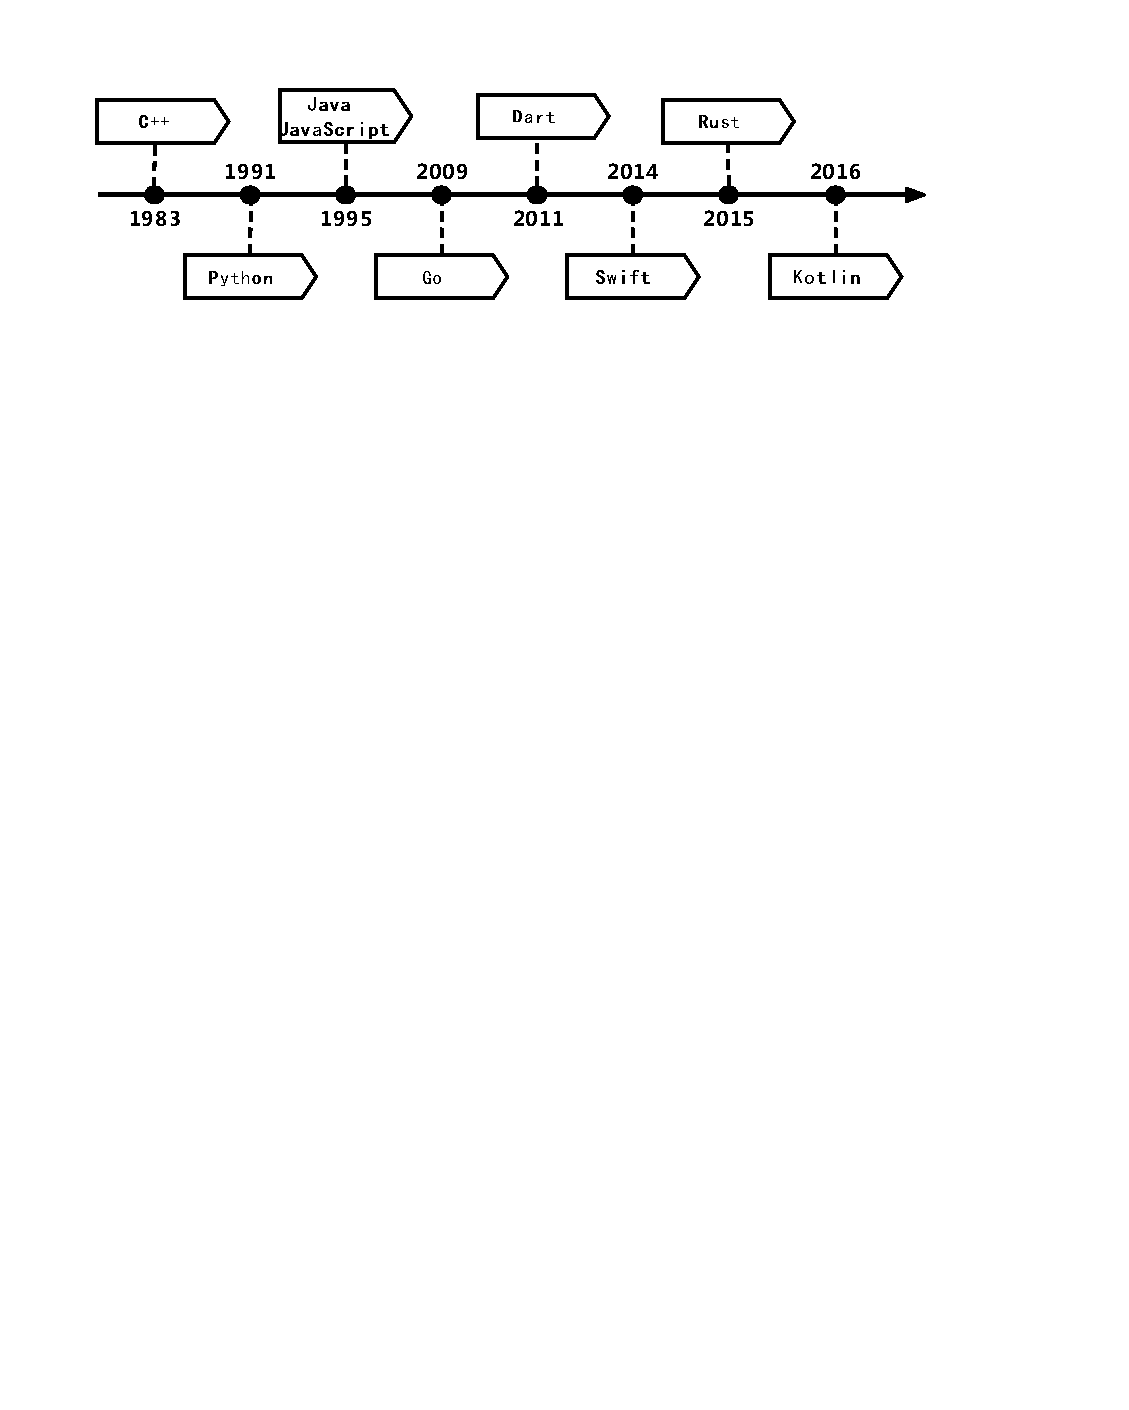
\includegraphics[scale=0.6]{figures/timeline}}
%    \caption{Timeline of several MPLs}
%    \label{fig:timeline}
%\end{figure}

%According to the data of the IEEE spectrum\cite{IEEETopProgrammingLanguages},
%the top five most popular programming languages in 2021 are Python, Java, C, C ++, and JavaScript. An exception case is C, which provides low-level access to computer systems. To be precise, the syntax design of the C language does not conform to any of the features of MPL. And for the four remaining popular programming languages mentioned above, they are still helpful even though they are not exactly in line with the features of MPL. In the era when these languages were first created, they emerged as representatives of MPLs. Therefore these four past programming languages are compared with the emerging MPLs.


%Based on the above-mentioned MPL features,
%several programming languages were selected and arranged
%in order of popularity\cite{IEEETopProgrammingLanguages},
%resulting in Go, Swift, Dart, Rust and Kotlin (where Swift and Dart are equally popular).
%%Coincidentally, these languages are also released in this order sequentially, see Figure\ref{fig:timeline}.
%%In addition, all of these languages have similar type systems and all support AOT compilation, and although not all use garbage collection memory management, they all move away from manual memory management.
%%These are all common features of MPLs in today's application environment, as we can see from Table\ref{tab:selected-languages}.

%\subsection{Criteria to evaluate the design of programming languages}


%We think there are two main aspects that determine whether a language is useful or not.
%One aspect is its syntactic design.
%For complex business logic, programming languages are required to provide
%strong expressiveness, i.e., isolate underlying implementations
%that are not related to the business logic to accommodate rapid changes.
%Programming languages are also needed to provide solutions for
%checking the correctness and reliability of programs.
%Another aspect is performance, where programming languages are
%always expected to have a low memory overhead and time overhead,
%relying heavily on compile-time (native languages) and run-time
%(virtual machine languages) optimizations.
%See Table\ref{tab:evaluate}.


We assess the designs of these MPLs from an application-oriented point of view.
In other words, we evaluate whether a language design is “practical”.
There are mainly two aspects that determine whether a language is practical or not.
One is its syntactic design.
To deal with complex business logic, programming languages are expected to be strong expressive,
which correlated with its paradigms.
%i.e., isolate underlying implementations that are not related to the business logic to
%accommodate rapid changes.
Programming languages also need to provide solutions for correctness checking,
which correlated with its type systems.
Ultimately, programming languages are always supposed to have a better performance,
which rely heavily on compile-time (native languages) and run-time (virtual machine languages) optimizations.
%Specifically, the evaluation criteria of this paper are presented in Table~\ref{tab:evaluate}.
%For expressiveness, maintainability, and reliability of a language, we analyze them
%by programming paradigm or type system;
%for Performance of a language, we analyze it by time overhead and memory overhead.
And the profile of the nine selected MPLs about their programming paradigm,
type system, compilation mode and memory model are shown in Table~\ref{tab:selected-languages}.

\begin{table*}[htbp]
    \caption{Several modern programming languages}
    \label{tab:selected-languages}
    \begin{center}
        \begin{tabular}{ccccccc}
            \toprule
            Language & Programming Paradigm & Type System & Compilation Mode & Memory Model &
            Release Date & Application Scenarios \\
            \midrule
            Python & Multi-paradigm & Dynamically, Strongly & JIT & GC & 1991 & Web,
            Enterprise, Embedded \\
            Java & Multi-paradigm & Statically, Strongly & AOT & GC & 1995 & Web,
            Mobile, Enterprise \\
            C++ & Multi-paradigm & Statically, Weakly & AOT & Manual & 1983 & Mobile,
            Enterprise, Embedded \\
            JavaScript & Multi-paradigm & Untyped & JIT & GC & 1995 &
            Web \\
            Go & Multi-paradigm & Statically, Strongly & AOT & GC & 2009 & Web,
            Enterprise \\
            Swift & Multi-paradigm & Statically, Strongly & AOT & ARC & 2014 &
            Mobile, Enterprise \\
            Dart & Multi-paradigm & Statically, Strongly & AOT\&JIT & GC & 2011 &
            Web, Mobile \\
            Rust & Multi-paradigm & Statically, Strongly & AOT & Ownership & 2015 &
            Web, Enterprise, Embedded \\
            Kotlin & Multi-paradigm & Statically, Strongly & AOT\&JIT & GC & 2016 &
            Web, Mobile \\
            \bottomrule
        \end{tabular}
    \end{center}
\end{table*}

%In practice, however, programming language design cannot be accurately quantified.
%The reason for this is twofold.
%The first is that certain criteria for evaluation are not quantitative.
%For expressiveness and reliability, both are abstract descriptions,
%and they have uncountable kinds of cases in practice.
%If one wants to analyze them quantitatively, then one must restrict the analysis to
%certain specific application scenarios.
%The second is that the evaluation criteria are not sufficient.
%Some evaluation criteria that are difficult to measure, such as response time in a
%real-time system, are dropped here for structural completeness.
%For programming languages with garbage collectors, the performance loss from garbage collection is not negligible. In particular, JVM-based programming languages have the problem of "Stop the World" when garbage collection is performed, which affects the performance of the programming language. However, this is not considered for the sake of simplicity.


%It should be emphasized that programming language design cannot be fully
%evaluated by quantitative analysis.
%For expressiveness and reliability, which are descriptions for abstract concepts,
%although quantitative analysis is possible, it is usually limited to a certain
%application environment, which does not have much significance.
%Some other performances are difficult to measure, such as response time in real-time systems.
%Additionally, for programming languages with garbage collectors, the performance
%loss from garbage collection is not negligible.
%In particular, JVM-based programming languages have the problem of "Stop the World"
%when garbage collection is performed\cite{gidra2013study},
%which affects the performance of the programming language.
%Such features are not considered in this paper.
    \section{Analysis of programming paradigms}

%By analyzing the degree of support of the nine MPLs
%for programming paradigms and the application scenarios of
%different MPLs, we try to find out the connection between
%the degree of support of programming paradigms and the
%application scenarios.

Extensive research has shown that programming is about solving problems,
and that problems can be solved from a variety of perspectives
and ideas, of which the universal and proven patterns are
summarized as paradigms.
Functional Programming (FP) and Object Oriented Programming (OOP)
are the two most common, and at the same time the most important paradigms
in modern programming languages.
Therefore, these two paradigms are chosen for analysis when discussing
programming paradigms below.

\subsection{Languages, paradigms, and concepts}



\begin{table*}[hb]
    \caption{Several concepts of FP and OOP}
    \label{tab:concept}
    \begin{center}
        \begin{tabular}{cll}
            \toprule
            Paradigm & Concept & Meaning \\
            \midrule
            FP & Higher-order function & Take functions as variables, which can
            pass as parameters or return values. \\
            FP & Lambda expression & A short block of code which takes in parameters
            and returns a value. \\
            FP & Partial application & Given a function with certain parameters,
            producing another function (with fewer parameters). \\
            FP & Closure & A record stores a function together with an
            environment\cite{sussman1998scheme}. \\
            FP & Type inference & The automatic detection of the type of an
            expression at compile time. \\
            FP & Pattern matching & Dispatch branch by matching the pattern of a
            given sequence of tokens. \\
            FP & Statement as expression & Take all statements as expressions, which
            creates a definite value. \\
            OOP & Encapsulation & Hide the properties and implementation details of
            the object, and only expose the interface to the outside. \\
            OOP & Inheritance & Create classes that are built upon existing
            classes\cite{johnson1988designing}. A way of
            code reuse. \\
            OOP & Composition & Combine entities into more complex ones. A way of
            code reuse. \\
            OOP & Delegation & One entity passing something to another
            entity\cite{wilkinson2009grid}. A way of code
            reuse. \\
            OOP & Trait & A set of method conventions. Broadly including trait,
            interface, protocol and mixin. \\
            OOP & Polymorphism & Use of a single symbol to represent multiple
            different
            types\cite{cardelli1985understanding}. \\
            OOP & Everything is object & All the basic elements of a programming
            language are represented in the form of objects. \\
            \bottomrule
        \end{tabular}
    \end{center}
\end{table*}

\begin{table*}[ht]
    \caption{Degree of support for FP concept}
    \label{tab:fp}
    \begin{center}
        \begin{tabular}{cccccccc}
            \toprule
            Language & Higher-order functions & Lambda expression & Partial
            application & Closures & Type inference & Pattern matching & Statements
            as expressions\\
            \midrule
            Python     & \Checkmark & \Checkmark & Python2.5   & \Checkmark & \Checkmark & Python3.10  & ×          \\
            Java       & Java8      & Java8      & Java8       & Java8      & Java10     & ×           & ×          \\
            C++        & C++11      & C++11      & C++11       & C++11      & C++11      & C++17       & ×          \\
            JavaScript & \Checkmark & \Checkmark & ECMAScript5 & \Checkmark & \Checkmark & ECMAScript6 & ×          \\
            Go         & \Checkmark & \Checkmark & \Checkmark  & \Checkmark & \Checkmark & ×           & ×          \\
            Swift      & \Checkmark & \Checkmark & \Checkmark  & \Checkmark & \Checkmark & \Checkmark  & ×          \\
            Dart       & \Checkmark & \Checkmark & \Checkmark  & \Checkmark & \Checkmark & ×           & ×          \\
            Rust       & \Checkmark & \Checkmark & \Checkmark  & \Checkmark & \Checkmark & \Checkmark  & \Checkmark \\
            Kotlin     & \Checkmark & \Checkmark & \Checkmark  & \Checkmark & \Checkmark & \Checkmark  & \Checkmark \\
            \bottomrule
        \end{tabular}
    \end{center}
\end{table*}

Each language also realizes one or more paradigms,
and each paradigm contains a core set of concepts,
as we can see in Table~\ref{fig:concept}.
FP and OOP are programming paradigms that are commonly
available in MPLs, so the rest of our discussion is based on FP and OOP\@.
Table~\ref{tab:concept} shows several concepts in FP and OOP supported by MPLs, and the meaning of a certain concept.

\begin{figure}[htbp]
    \centerline{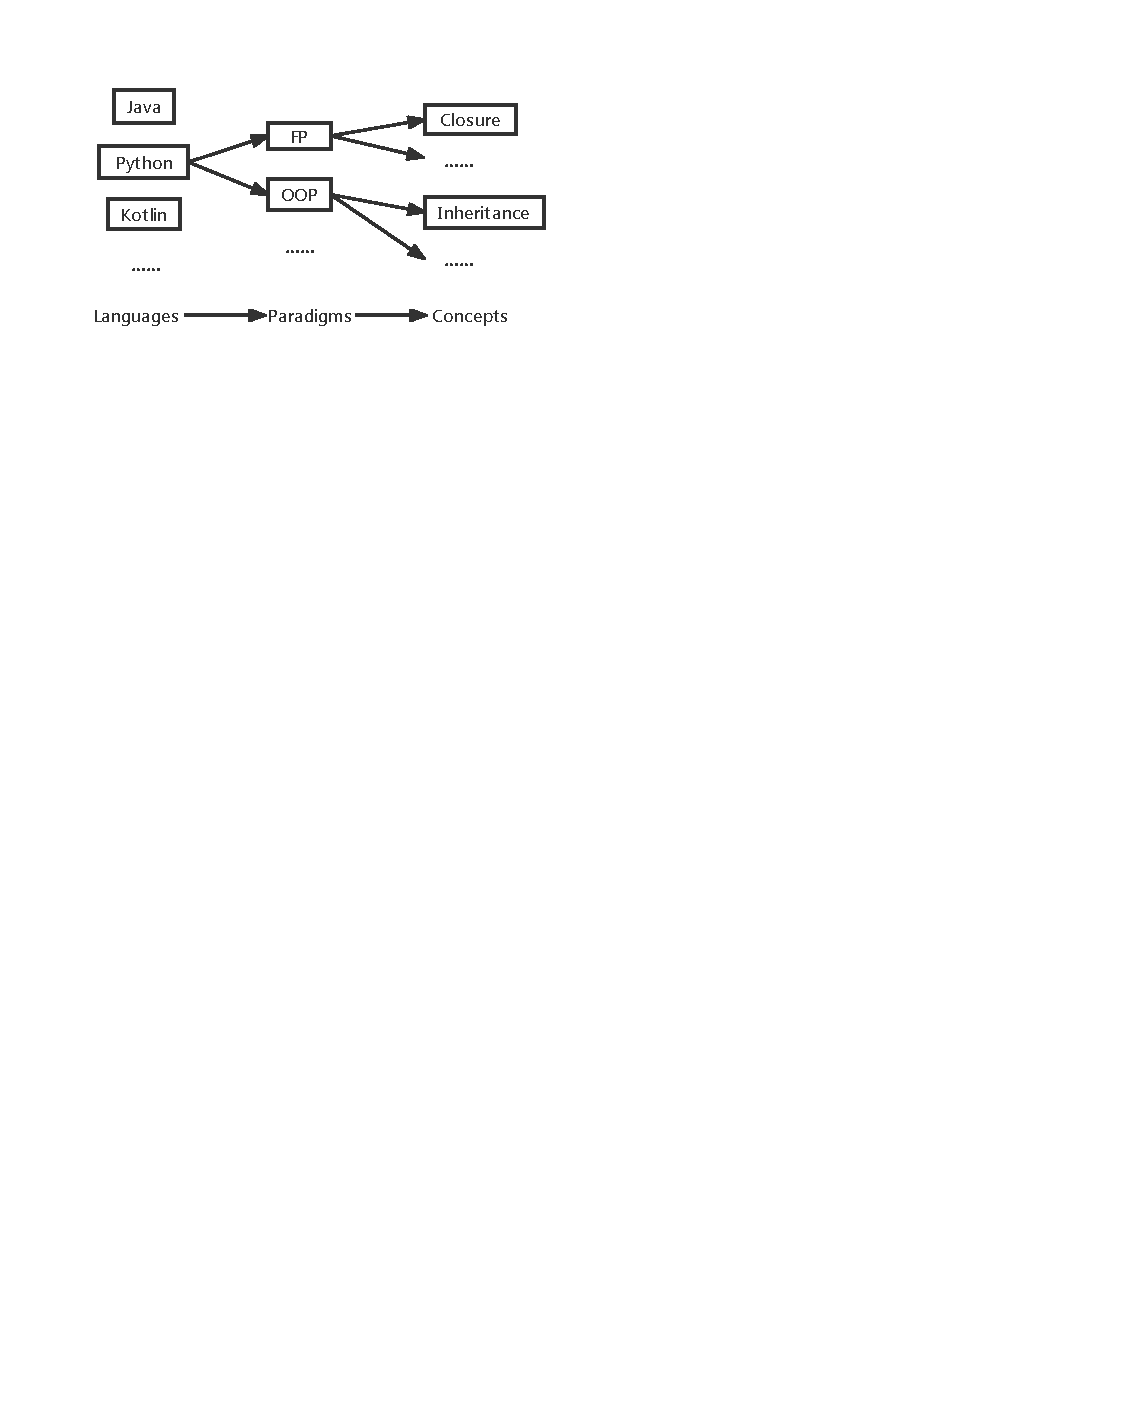
\includegraphics[scale=0.8]{figures/concept}}
    \caption{Languages, paradigms, and concepts}
    \label{fig:concept}
\end{figure}


We have adopted a more application-oriented approach to concept organization.
It will tend to choose concepts defined in a particular programming
language rather than concepts from programming paradigm theory.
For example, for the functional concept of nested and anonymous functions,
they are implemented as lambda expressions in many programming languages.
As another example, most of the currently popular programming languages
support combinations in the object-oriented concept.
When designing programming languages, combinations are simply a way of
arranging data and do not belong to any paradigm.
Even languages like the much older C provide structure combinations and
function combinations.
Therefore, combinations are not included in the analysis.

\subsection{Functional programming}

The most important feature of FP is its high degree of abstraction.
This is mainly because FP has its origins in the lambda calculus,
so it has some characteristics of abstract algebra.


As programming language practice continues to deepen,
programming languages are becoming more and more supportive
of functional concepts.
Table~\ref{tab:fp} gives the support level of the selected 9 MPLs for the concepts
of FP mentioned in Table~\ref{tab:concept}.
The right/wrong signs indicate that the programming language has
supported/not supported the concept since the beginning,
and if the programming language has supported a concept during its development,
the version that first supported the concept is indicated.


For programming languages released in the 1980s and 1990s,
the support for functional concepts was not good when they
were first created.
This is especially true for Java and C++.
From the original syntax, one did not design them with FP in mind.
And for JavaScript and Python, they are a bit better in this regard.
Although they inherently support some functional concepts,
they are still missing some advanced functional concepts.
As for the programming languages released around 2010,
they all support the basic functional concept.
In particular, Rust and Kotlin additionally support the concept
of "statements as expressions", a milestone in the development
of MPL paradigm convergence.
The concept of "statements as expressions"
is more common in functional languages and provides semantic
unification of expressions and statements.
However, this concept is not supported in most programming languages with paradigm convergence.
As programming languages continue to evolve, Kotlin and Rust
are supporting this concept with paradigm convergence.
Thus Kotlin and Rust can be considered as having a higher
level of support for FP concepts.

\subsection{Object oriented orogramming}
The most important feature of OOP is its emphasis on reuse. Back in the 1960s, software maintenance became increasingly difficult due to the increasing complexity of hardware and software. OOP solves this problem by emphasizing reusability. In the practice of OOP, one maps real problems into entities and their relationships, rather than being concerned with the process of dealing with the problem.

%The most important feature of OOP is its emphasis on reuse. Back in the 1960s, software maintenance became increasingly difficult due to the increasing complexity of hardware and software. OOP solves this problem by emphasizing reusability. In the practice of OOP, one maps real problems into entities and their relationships, rather than being concerned with the process of dealing with the problem. After the birth of object-oriented languages, there was an urgent need to map from problems to entities and relationships in a modeling way, at which point UML was born. It is a set of standardized modeling languages for visualization and has greatly contributed to the development of object-oriented methodologies. Since then the practice of OOP has always emphasized design before implementation.

For the core concepts of OOP, there is not much difference in the level of support of MPLs, see Table~\ref{tab:oop}.
Table~\ref{tab:oop} shows the degree of support of the selected 9 MPLs for the conception of the OOP
mentioned in Table~\ref{tab:concept}.
The meaning of the right/wrong signs in the table is the same as in Table~\ref{tab:fp}.

There are three ways to realize reuse: inheritance, combination, and delegation.
In addition, more and more programming languages are realizing object-oriented
features by supporting combinations and delegates, while mere
inheritance has proven to be bad practice\cite{gamma1995design}.
Therefore, the concept of classes and inheritance is abandoned in Go and Rust, and object orientation is realized through trait. Compared to class-based object-oriented, trait-based object-oriented has a looser coupling and more flexible realization. However, most MPLs support both trait and class for different granularity of control.

In order to more accurately distinguish the degree of OOP concept support for each MPL, some concepts that are not commonly used are introduced here. An example is "everything is object". According to the definition of OOP, it should have been the most basic concept in OOP. In fact, however, early programming languages tended to have a large number of imperative features, i.e., not all elements were treated as objects. For example, there are still primitive data types in Java, which are not objects, so we cannot call methods of these types as if they were objects. Perhaps there are many performance positives of primitive data types, but from a semantic consistency perspective, primitive data types have negative effects. Therefore, languages with the concept of "everything is object" are considered to have a higher level of OOP support.

\begin{table*}[htbp]
    \caption{Degree of support for OOP concept}
    \label{tab:oop}
    \begin{center}
        \begin{tabular}{cccccc}
            \toprule
            Language & Inheritance & Delegation & Traits & Polymorphism &
            Everything is object \\
            \midrule
            Python     & \Checkmark & \Checkmark & ×          & \Checkmark & \Checkmark \\
            Java       & \Checkmark & ×          & \Checkmark & \Checkmark & ×          \\
            C++        & \Checkmark & ×          & \Checkmark & \Checkmark & ×          \\
            JavaScript & \Checkmark & \Checkmark & ×          & \Checkmark & \Checkmark \\
            Go         & ×          & ×          & \Checkmark & \Checkmark & ×          \\
            Swift      & \Checkmark & ×          & \Checkmark & \Checkmark & \Checkmark \\
            Dart       & \Checkmark & ×          & ×          & \Checkmark & \Checkmark \\
            Rust       & ×          & \Checkmark & \Checkmark & \Checkmark & \Checkmark \\
            Kotlin     & \Checkmark & \Checkmark & \Checkmark & \Checkmark & \Checkmark \\
            \bottomrule
        \end{tabular}
    \end{center}
\end{table*}

\subsection{Programming Paradigms and Applications}

We try to find the relationship between the degree of programming language support for
programming paradigms and the application scenarios of the programming language.
By combining Table~\ref{tab:fp} and Table~\ref{tab:oop} and the results of their analysis, we obtain Figure~\ref{fig:paradigm}.
The x-axis and y-axis in Figure~\ref{fig:paradigm} represent respectively
the degree of OOP and FP support of the programming language.
The larger its coordinate on the x-axis, the better its support for OOP.
Similarly, the larger its coordinate on the y-axis, the better its support for FP.
Based on our analysis of the support level of programming paradigm above,
we partitioned the support level of FP into three levels and the support level of OOP into two levels.
Programming languages that have the same level, we consider that they have similar programming paradigms.
What is clear is that Kotlin and Rust have the best level of FP and OOP support.
Meanwhile, C++ and Java have the worst support.
We can see that, in general, the later the release of a programming language,
the better its support for FP and OOP.

\begin{figure}[htbp]
    \centerline{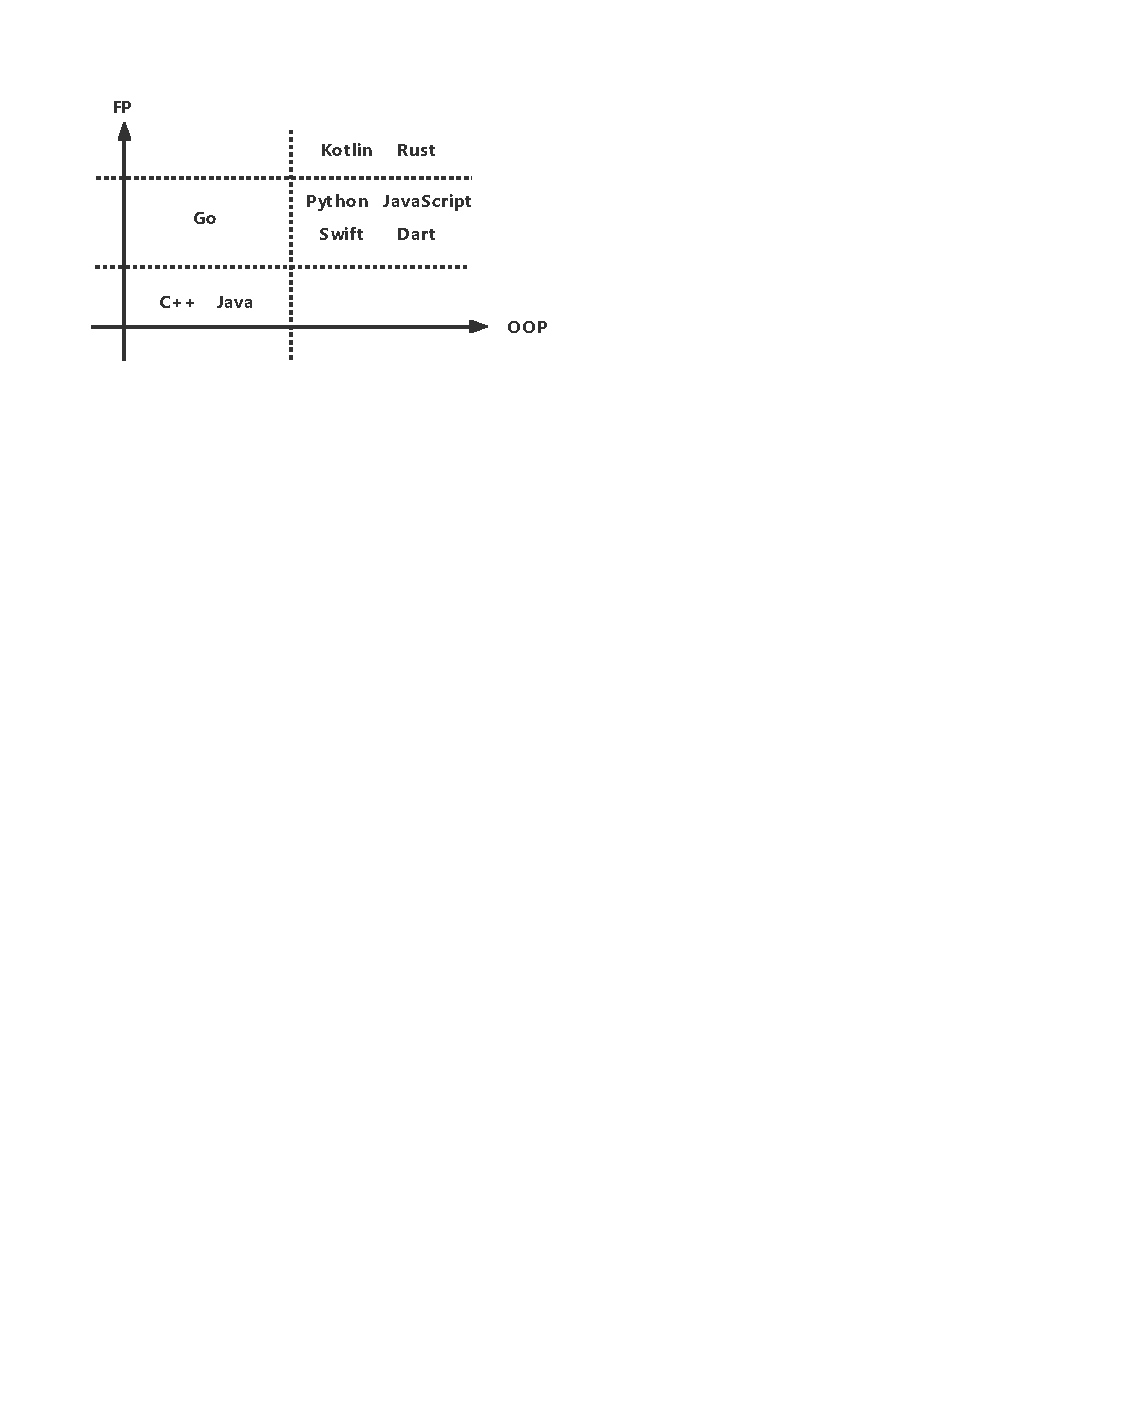
\includegraphics[scale=0.8]{figures/paradigm}}
    \caption{Degree of programming paradigm concept support}
    \label{fig:paradigm}
\end{figure}

The degree to which a programming language supports a programming paradigm is closely related
to the application scenario of the programming language.
Next, we will select a few representative programming languages from Figure~\ref{fig:paradigm} and analyze the
relationship between their programming paradigms and application scenarios.


A typical example is Dart. Its main application scenario is the Web front-end, and it is often used as a support language for the GUI framework Flutter. It is obvious that most of the GUI frameworks we use have a complex inheritance structure. This is because, for GUIs, most of its application scenarios satisfy the Liskov Substitution Principle, i.e., the child type can completely replace the parent type. This is a sufficient condition for using inheritance. Therefore, Dart only provides object-oriented concepts based on inheritance.

The next example is Java, which has weak support for both FP and OOP concepts. In the early years, Java was used for Enterprise development. Later it was used for Web servers, a scenario that required high abstraction of business logic, so Java added the additional concept of FP. However, due to the design of the language itself, the level of support is not high.

Another example is Kotlin, which has better support for both FP and OOP. Its initial application scenario is Android. In order to solve the previous problem that Java was too cumbersome to develop Android applications, Kotlin was designed to add a lot of FP and OOP concepts for the Android application scenario. Not only does it support traditional FP and OOP concepts, but it also makes syntax-level optimizations for these concepts, such as the FP syntactic sugar "trailing lambda" and the OOP delegate syntactic sugar "by". These useful features in turn allow Kotlin to be used in other scenarios, such as server front-ends and back-ends.
    \section{Analysis of type system}

\begin{figure}[htbp]
    \centerline{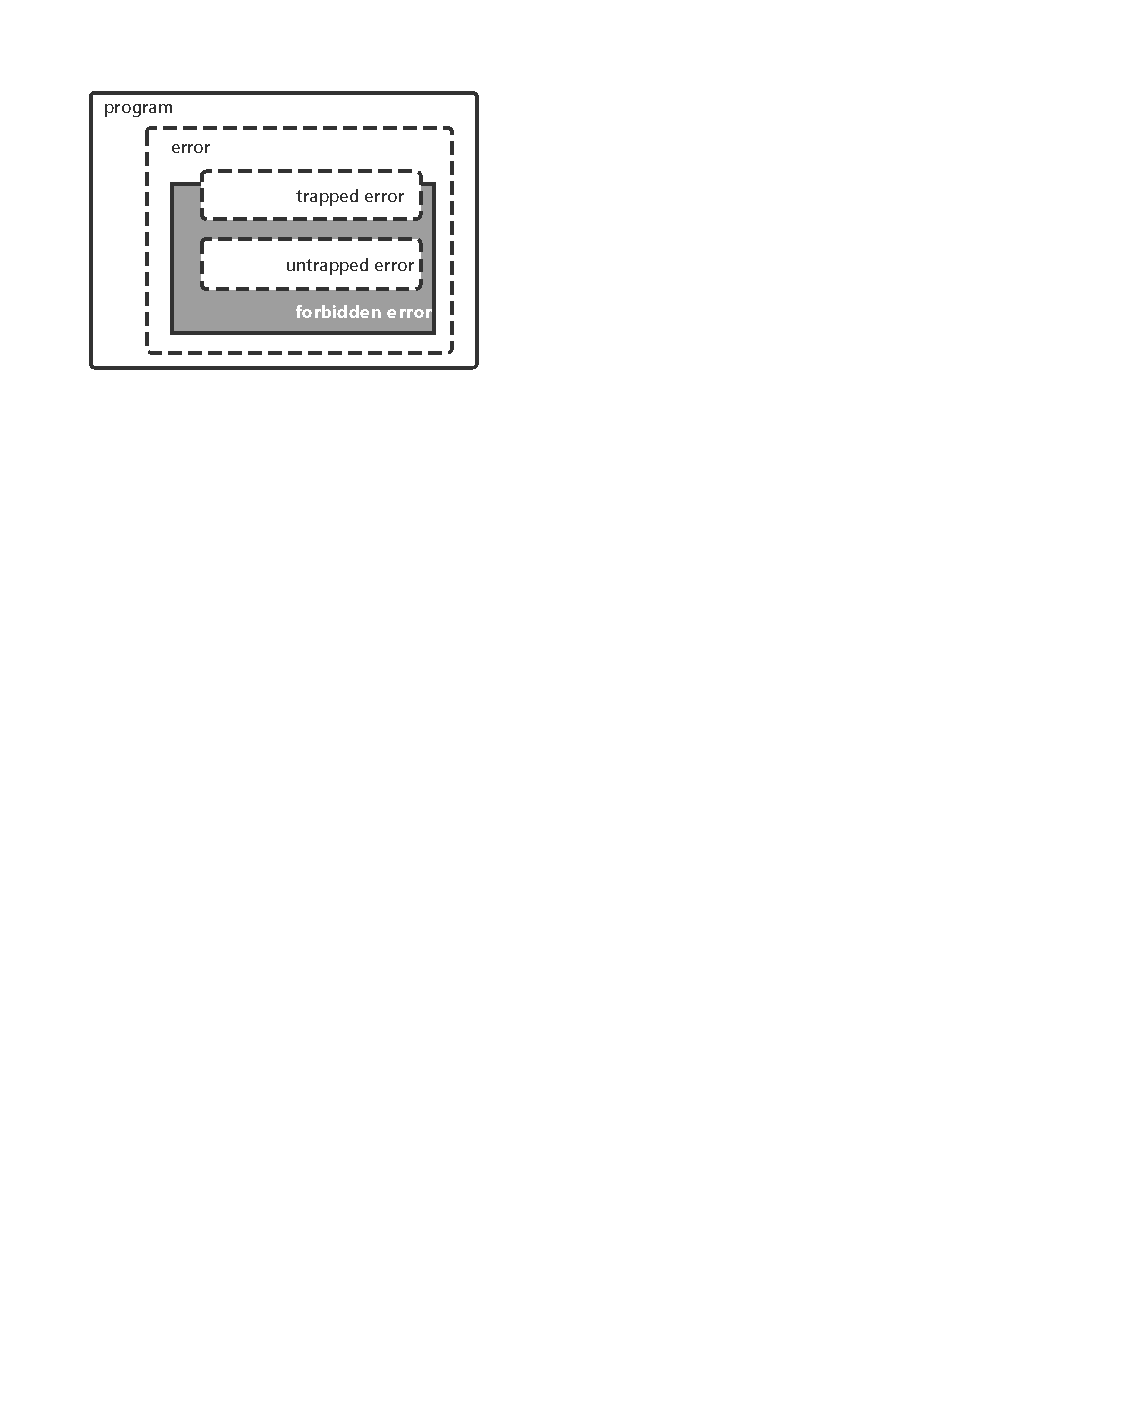
\includegraphics[scale=0.8]{figures/type-definition}}
    \caption{Definition of forbidden error}
    \label{fig:type-definition}
\end{figure}


\begin{table*}[htbp]
    \caption{Several type systems of MPLs}
    \label{tab:type}
    \begin{center}
        \begin{tabular}{cccccc}
            \toprule
            Language & Typed/Untyped & Explicitly/Implicitly typed &
            Dynamically/Statically checked & Strongly/Weakly checked & Well behaved\\
            \midrule
            Python     & Typed   & Implicitly & Dynamically & Strongly & Yes \\
            Java       & Typed   & Explicitly & Statically  & Strongly & Yes \\
            C++        & Typed   & Explicitly & Statically  & Weakly   & No  \\
            JavaScript & Untyped & -          & Dynamically & -        & Yes \\
            Go         & Typed   & Explicitly & Statically  & Strongly & Yes \\
            Swift      & Typed   & Explicitly & Statically  & Strongly & Yes \\
            Dart       & Typed   & Explicitly & Statically  & Strongly & Yes \\
            Rust       & Typed   & Explicitly & Statically  & Strongly & Yes \\
            Kotlin     & Typed   & Explicitly & Statically  & Strongly & Yes \\
            \bottomrule
        \end{tabular}
    \end{center}
\end{table*}


The discussion here is based on L. Cardelli's definition of type systems\cite{cardelli1996type}.
This definition considers that the fundamental purpose of
the type system is to prevent errors that occur during the
runtime of a program, and therefore defines the type system by defining
concepts related to errors.
According to Figure~\ref{fig:type-definition}, there are two types of errors.
An error that immediately results in a fault is called a trapped error.
The other will not cause fault immediately, called untrapped error.
All untrapped errors and some trapped errors are collectively
called forbidden errors.


programming languages are divided into (statically) typed languages and (statically) untyped languages
depending on whether they have static types to limit the scope of variable types at runtime.
Based on the timing of behavior checking, programming languages
can be classified as statically checked languages and Dynamically checked languages.
On the basis of statically checked languages, languages that cannot check out
all forbidden errors are called weakly typed languages.
Conversely, it is called strong checked language.
Then explicitly typed languages and implicitly typed languages are
classified according to whether the programming language explicitly
specifies the type of the variable.
A program is said to have good behavior if it does not produce
forbidden errors during execution.
According to the above definition,
we have analyzed and got the Table~\ref{tab:type}.

There is one thing to note.
Type hints were introduced in Python in version 3.5.
But type hints do not actually do error checking for Python.
It is simply a type annotation to help provide better support
for static analysis syntax parsers.
The real time for error checking is still at runtime.
So Python is still a dynamically typed, strongly typed language.

Table~\ref{tab:type} gives the type system of common MPLs according
to L Cardelli's type system definition.
It is worth noting that most current MPLs have certain commonalities.
They are often explicitly typed, strongly typed, statically typed, and well-behaved.
This is inseparable from the application areas of these languages.
Type signatures contain constraint information by which the behavior of
variables or functions can be indirectly determined.
It improves maintainability, which is exactly what programming languages
for industrial applications need.
Static type checking and formal proofs of type systems improve the reliability
of programs and help people write less error-prone code.
Also, a static type system is more conducive to performance optimization
and memory allocation, and object programs can have better performance.

    \section{Analysis of performance}

To more accurately measure the performance of each language, we introduce benchmarking.

In computer science, benchmarking refers to the evaluation of
the performance of an object by running a computer program or
manipulating some specific behavior\cite{fleming1986not}.
It is done through a series of comparative experiments with
controlled variables usually involving several iterative rounds
in order to draw reproducible and precise conclusions.
In addition, it focuses on a particular procedure and
should exclude the influence of unrelated procedures on
the benchmark test.
This requires that the benchmark test should have a
clear idea of how the underlying workings work and avoid errors
due to the uncertainty of the system's state.

\subsection{Benchmarking Setup}

%\begin{table}[htb]
%    \centering
%    \caption{Benchmarking platform}
%    \label{tab:platform}
%    \begin{tabular}{cc}
%        \hline
%        CPU    & ECS 4 Cores 3.0GHz \\
%        Memory & 16GiB              \\
%        OS     & CentOS 8.2 64bit   \\
%        \hline
%    \end{tabular}
%\end{table}

This test uses Python scripts to perform coarse-grained
batch testing uniformly and uses built-in process tools
to invoke Linux system commands without relying on
third-party libraries, which has high testing efficiency
and is, therefore, suitable for large amounts of data.
Each test program was executed six times, and the results
were averaged to avoid bias.
Each benchmark test was
executed with larger and smaller scale inputs.
We choose the host with a 4-core 3.0GHz CPU, 16GB RAM, CentOS 8.2.
For the compiler environment of the programming
language, see Table\ref{tab:version}.

\begin{table}[htbp]
    \caption{Language versions and dependencies}
    \label{tab:version}
    \begin{center}
        \begin{tabular}{ccc}
            \toprule
            Language   & Version         & Dependency \\
            \midrule
            Python     & CPython3.8      & -          \\
            Java       & OpenJDK17       & -          \\
            C++        & Clang14/GCC11.2 & -          \\
            JavaScript & Node16          & -          \\
            Go         & Go1.17          & -          \\
            Swift      & Swift5.5        & -          \\
            Dart       & Dart2.16        & -          \\
            Rust       & Rust1.54        & MinGW7.3   \\
            Kotlin     & Kotlin1.6       & OpenJDK8   \\
            \bottomrule
        \end{tabular}
    \end{center}
\end{table}

For the same language with different compilers or compilation methods, compare their differences (e.g. C++, Dart). For the remaining languages, we classify them according to the programming language type system. Because for multiple languages with the same type system and compilation method, there should be overlap in their scope of application in practice, the comparative analysis.

The benchmarking metrics for computer languages come from one of the
more popular cross-language benchmarking suites available -
the Computer Language Benchmarking Game\cite{gouy2017computer}.
For each language, there are four metrics.


\begin{enumerate}
    \item Compiler. marked after the programming language, if not marked then the official compiler is used.
    \item Size. The size of the source code after gzip compression. For the same algorithm, the smaller the amount of code used by a programming language, the more syntactically expressive the language is, in general.
    \item CPU. The time required to run the algorithm. Takes the minimum value of multiple runs. Includes startup time.
    \item Memory. The peak space consumption to run the algorithm. Takes the maximum of multiple runs.
\end{enumerate}

\subsection{Memory allocation test}
The idea is derived from Hans-J. Boehm's GC bench algorithm.
The memory allocation capacity and garbage collection capacity are measured by repeatedly allocating and deallocating large amounts of space.
The steps are described in Algorithm 1.
We obtain the CPU and memory overhead results for the selected MPLs
by taking n=21 and n=14, respectively, as shown in Table~\ref{tab:binary-trees-1} and Table~\ref{tab:binary-trees-2}.

\begin{figure}[htbp]
    \centerline{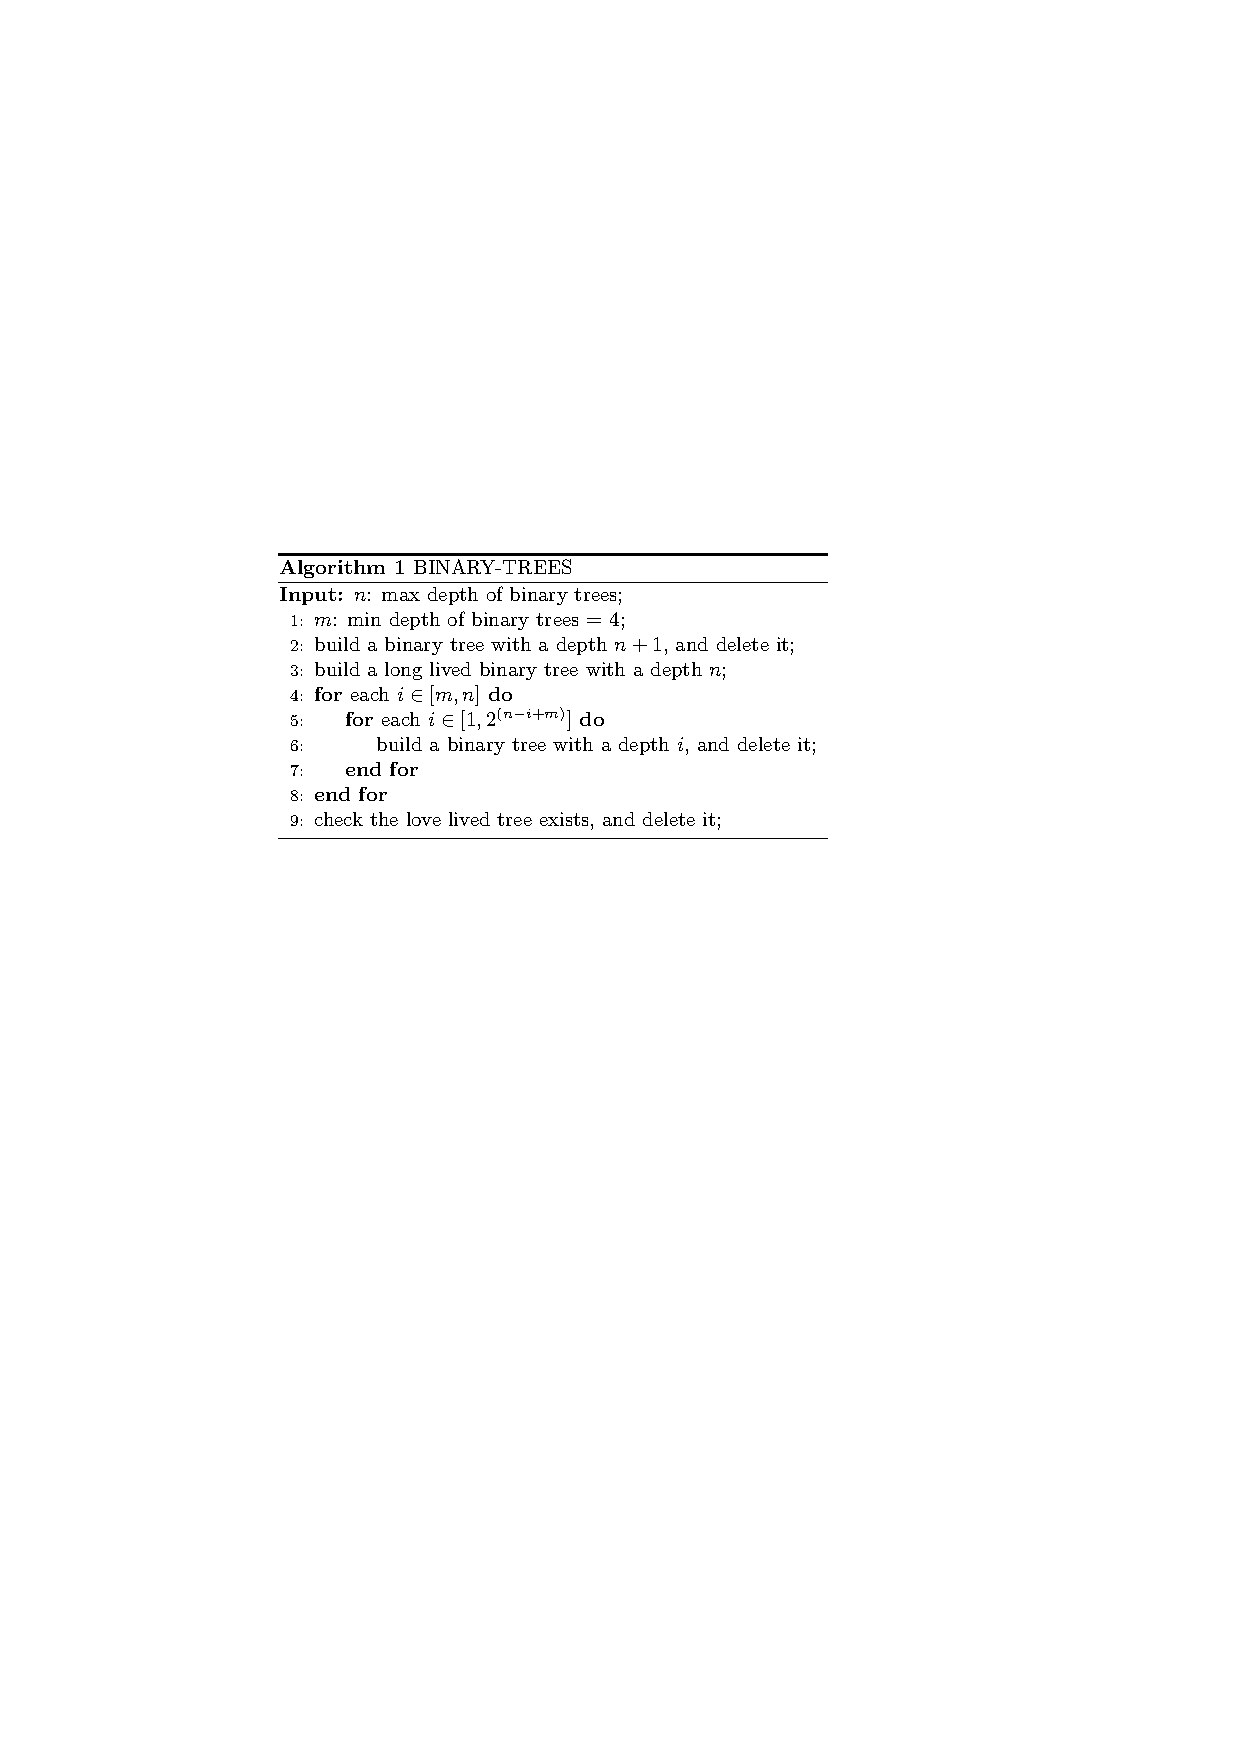
\includegraphics[scale=0.8]{figures/binary-trees}}
    \label{fig:binary-trees}
\end{figure}

\begin{table}[ht]
    \caption{Memory allocation test - large input}
    \label{tab:binary-trees-1}
    \begin{center}
        \begin{tabular}{lrrrr}
            \toprule
            lang      & n  & size(B) & cpu(s)  & mem(KB) \\
            \midrule
            cpp-clang & 21 & 654     & 16.438  & 263580  \\
            cpp-gcc   & 21 & 654     & 22.181  & 263620  \\
            dart-aot  & 21 & 1212    & 45.461  & 799012  \\
            dart-jit  & 21 & 1212    & 61.531  & 1626352 \\
            go        & 21 & 482     & 50.955  & 220548  \\
            java      & 21 & 552     & 5.607   & 2015512 \\
            js-node   & 21 & 711     & 36.391  & 1130788 \\
            kt-jvm    & 21 & 494     & 8.923   & 1783144 \\
            python3   & 21 & 589     & 169.912 & 442180  \\
            rust      & 21 & 751     & 7.796   & 132508  \\
            swift     & 21 & 714     & 63.608  & 733144  \\
            \bottomrule
        \end{tabular}
    \end{center}
\end{table}

\begin{table}[htbp]
    \caption{Memory allocation test - small input}
    \label{tab:binary-trees-2}
    \begin{center}
        \begin{tabular}{lrrrr}
            \toprule
            lang      & n  & size(B) & cpu(s) & mem(KB) \\
            \midrule
            cpp-clang & 14 & 654     & 0.087  & 1200    \\
            cpp-gcc   & 14 & 654     & 0.104  & 3928    \\
            dart-aot  & 14 & 1212    & 0.120  & 1680    \\
            dart-jit  & 14 & 1212    & 0.644  & 170008  \\
            go        & 14 & 482     & 0.214  & 7232    \\
            java      & 14 & 552     & 0.155  & 47968   \\
            js-node   & 14 & 711     & 0.717  & 90512   \\
            kt-jvm    & 14 & 494     & 0.249  & 36040   \\
            python3   & 14 & 589     & 0.911  & 14420   \\
            rust      & 14 & 751     & 0.042  & 1176    \\
            swift     & 14 & 714     & 0.299  & 17616   \\
            \bottomrule
        \end{tabular}
    \end{center}
\end{table}

As we can see from the Table\ref{tab:binary-trees-1} and Table~\ref{tab:binary-trees-2},
Java has the best memory allocation and management
speed among these programming languages.
However, Java's memory consumption is relatively the largest among these languages.
This is due to the unique memory model of the JVM, which divides the heap area into
different generations and uses different garbage collection algorithms for each generation.
The advantage of this is obvious, it can greatly increase the efficiency of garbage
collection. But at the same time, it takes up more memory than is actually needed for the division.
Since Kotlin and Java are both based on the JVM, they have similar performance figures.
Kotlin is based on Java8, while Java is based on Java17. From Java9 onwards, the default JVM GC is G1.
It has better response time than Parallel, but consumes more memory at the same time.
This is in line with the data in the table that Kotlin's time overhead is slightly higher
than Java's and memory overhead is slightly lower.

In Table~\ref{tab:binary-trees-1} and Table~\ref{tab:binary-trees-2},
for the two different compilers for C++, Clang and GCC, the memory overhead is almost the same.
This is because both of them manage memory manually.
However, Clang has a lower time overhead than GCC. This comes from compiler optimizations,
and Clang's optimizations are better than GCC's. In addition, the architecture of the compilers is different:
Clang-LLVM uses a low-coupling front- and back-end architecture, while GCC uses a front- and back-end coupling
architecture.
We can see that compile-time optimization of the compiler takes a more important role for native compiled languages.

Rust, Go and Swift, which are also strongly typed, natively compiled MPLs,
use three different memory management models.
The test results for all three are highly dependent on their
respective memory models.
Go uses a garbage collector.
Although Go is a natively compiled language, there is an additional runtime to support garbage collection.
Compared to Java, Go uses a more conservative garbage collection strategy and does
not aggressively use a space-for-time approach, resulting in decent space consumption
and less optimistic runtimes for memory allocation in Table~\ref{tab:binary-trees-1} and Table~\ref{tab:binary-trees-2}.
Rust uses an ownership mechanism,
unlike C/C++, which is purely manually managed, and unlike Go's garbage collection.
In terms of the underlying implementation, Rust does not actually maintain a runtime
to manage space but rather determines the timing of unallocating memory at compile
time through a complex arithmetic ownership algorithm. As a result, Rust's memory
management is overhead-free. In fact, Rust's compiler backend uses LLVM, the same
backend as the Clang-LLVM tested above, and it is also clear from the test data that
Rust performs almost identically to Cpp-Clang in Table~\ref{tab:n-body-1} and Table~\ref{tab:n-body-2}.
However,due to its ownership mechanism, Rust is better at memory allocation. For Swift,
the memory management mechanism is different from all of the above. Swift allocates
and deallocates memory by maintaining a runtime reference count. In addition,
Swift forces reference counts to be updated atomically instead of Rust's compiler
management of thread safety, which results in high CPU overhead in Table~\ref{tab:binary-trees-1} and Table~\ref{tab:binary-trees-2}. This shows that
Swift has a higher runtime overhead compared to Rust, confirming the data that
Swift performs poorly compared to Rust.

\subsection{Floating-point operation test}

The idea comes from the Symplectic Integration algorithm of K. P. Rauch
and D. P. Hamilton.
This algorithm simulates the evolution of multiple planets and checks the correctness of the program by examining the energy of each evolutionary state. The performance bottleneck is mainly in floating-point operations.
The steps are described in Algorithm 2.
We obtain the CPU and memory overhead results
for the selected MPLs by taking n=5e7 and n=5e6, respectively,
as shown in Table~\ref{tab:n-body-1} and Table~\ref{tab:n-body-2}.

\begin{figure}[htbp]
    \centerline{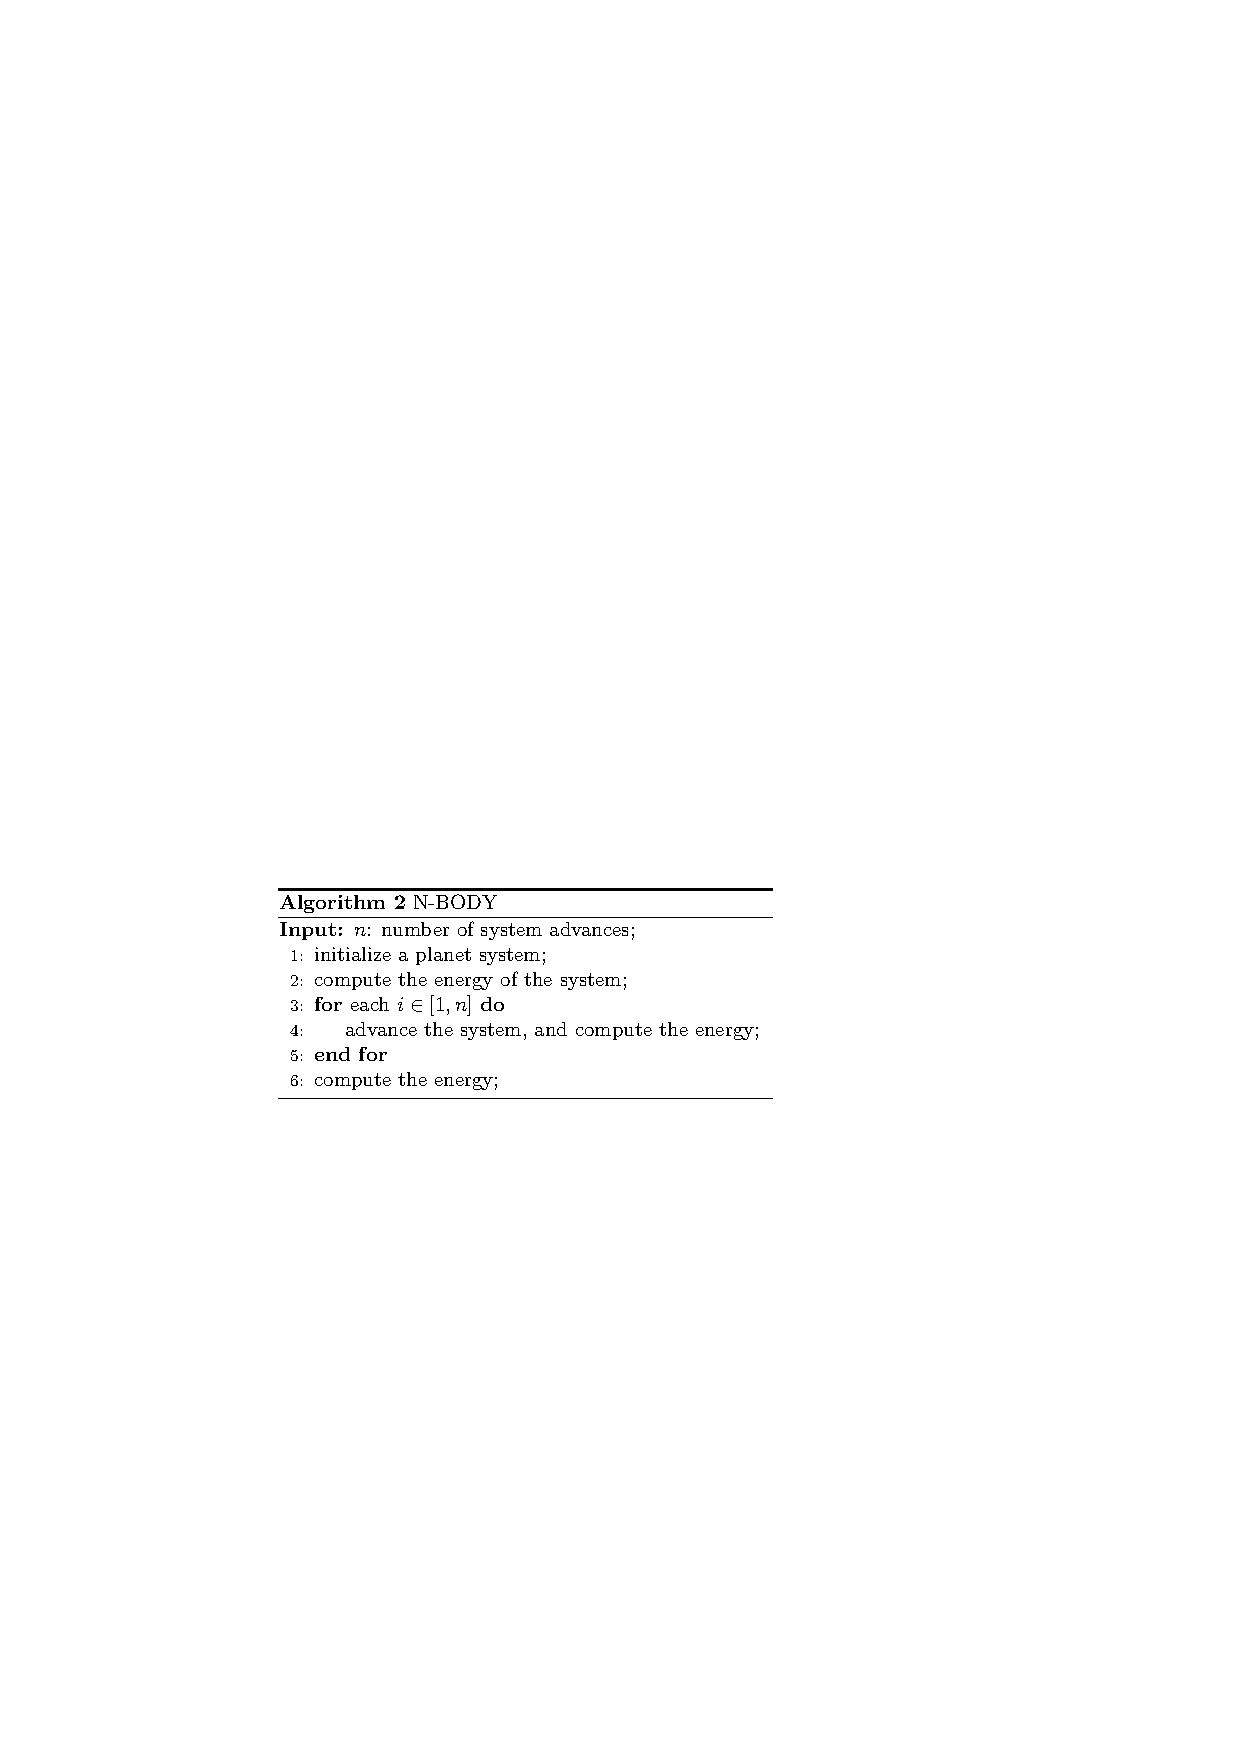
\includegraphics[scale=0.8]{figures/n-body}}
    \label{fig:n-body}
\end{figure}

\begin{table}[ht]
    \caption{Floating-point operation test - large input}
    \label{tab:n-body-1}
    \begin{center}
        \begin{tabular}{lrrrr}
            \toprule
            lang      & n        & size(B) & cpu(s)  & mem(KB) \\
            \midrule
            cpp-clang & 50000000 & 1173    & 5.926   & 1236    \\
            cpp-gcc   & 50000000 & 1173    & 7.555   & 1228    \\
            dart-aot  & 50000000 & 1266    & 10.220  & 9308    \\
            dart-jit  & 50000000 & 1266    & 13.193  & 143436  \\
            go        & 50000000 & 1310    & 6.581   & 1128    \\
            java      & 50000000 & 1430    & 7.816   & 37260   \\
            js-node   & 50000000 & 1268    & 8.550   & 39956   \\
            kt-jvm    & 50000000 & 1124    & 6.914   & 37068   \\
            python3   & 50000000 & 1196    & 541.319 & 7780    \\
            rust      & 50000000 & 1480    & 5.818   & 1024    \\
            swift     & 50000000 & 1192    & 9.585   & 6308    \\
            \bottomrule
        \end{tabular}
    \end{center}
\end{table}


\begin{table}[htbp]
    \caption{Floating-point operation test - small input}
    \label{tab:n-body-2}
    \begin{center}
        \begin{tabular}{lrrrr}
            \toprule
            lang      & n       & size(B) & cpu(s) & mem(KB) \\
            \midrule
            cpp-clang & 5000000 & 1173    & 0.621  & 1204    \\
            cpp-gcc   & 5000000 & 1173    & 0.766  & 1204    \\
            dart-aot  & 5000000 & 1266    & 1.033  & 9216    \\
            dart-jit  & 5000000 & 1266    & 1.918  & 143256  \\
            go        & 5000000 & 1310    & 0.661  & 816     \\
            java      & 5000000 & 1430    & 0.880  & 37460   \\
            js-node   & 5000000 & 1268    & 0.941  & 39864   \\
            kt-jvm    & 5000000 & 1124    & 0.826  & 37064   \\
            python3   & 5000000 & 1196    & 52.530 & 7800    \\
            rust      & 5000000 & 1480    & 0.579  & 1020    \\
            swift     & 5000000 & 1192    & 0.976  & 6308    \\
            \bottomrule
        \end{tabular}
    \end{center}
\end{table}

In Table~\ref{tab:binary-trees-1} and Table~\ref{tab:binary-trees-2},
Java's time overhead is not very high and does not fall too far behind natively compiled languages. The performance bottleneck of algorithmic programs with short execution time is mainly the JVM startup time and the JIT-optimized warm-up time, and for algorithms that have already done so, Java's execution speed does not lag behind that of natively compiled languages. Java runs in two steps. In the first step, the source code is compiled into bytecode, and in the second step, the JVM interprets and executes the bytecode. In the process of interpreting and executing the bytecode, JVM will receive the runtime information of the collected code, and if it finds that some bytecode is executed more frequently, it will choose to compile this part of the bytecode and compile it into native code, which will be called directly when it is executed again. The so-called performance optimization of Java is mainly in the bytecode, while the source to bytecode stage is only a simple optimization.

In Table~\ref{tab:binary-trees-1} and Table~\ref{tab:binary-trees-2},
there is a significant performance gap between JavaScript and Python. JavaScript runs on Google's V8 engine, which executes JavaScript code much like the JVM executes bytecode, using the same JIT optimization technique. So compared to Python, which does not use JIT optimization, it has a huge performance improvement, even with Java and natively compiled languages with similar floating point performance. In fact, the speed of scripting languages is not a performance bottleneck in most application scenarios. However, in recent years, JavaScript has become the "assembly of the web", and more and more languages are being compiled into JavaScript, such as Kotlin and Dart, so more and more business logic needs to be executed in JavaScript. This makes JavaScript burdened with tedious business-related logic, and optimization of JavaScript is the trend.

\subsection{Comprehensive test}

The Mandelbrot Set is drawn on a resolution N×N bitmap. the coordinates of the image on the complex axis are [-1.5-i,0.5+i]. For each pixel, a certain number of iterations are performed to determine the gray level of the current pixel. The output in PBF format is performed byte by byte. The correctness is checked by comparing it with the standard output. The performance bottleneck of this test is in floating point operations, memory allocation, and IO.
The steps are described in Algorithm 3.
We obtain the CPU and memory overhead results
for the selected MPLs by taking n=16000 and n=4000, respectively,
as shown in Table~\ref{tab:mandelbrot-1} and Table~\ref{tab:mandelbrot-2}.

\begin{figure}[htbp]
    \centerline{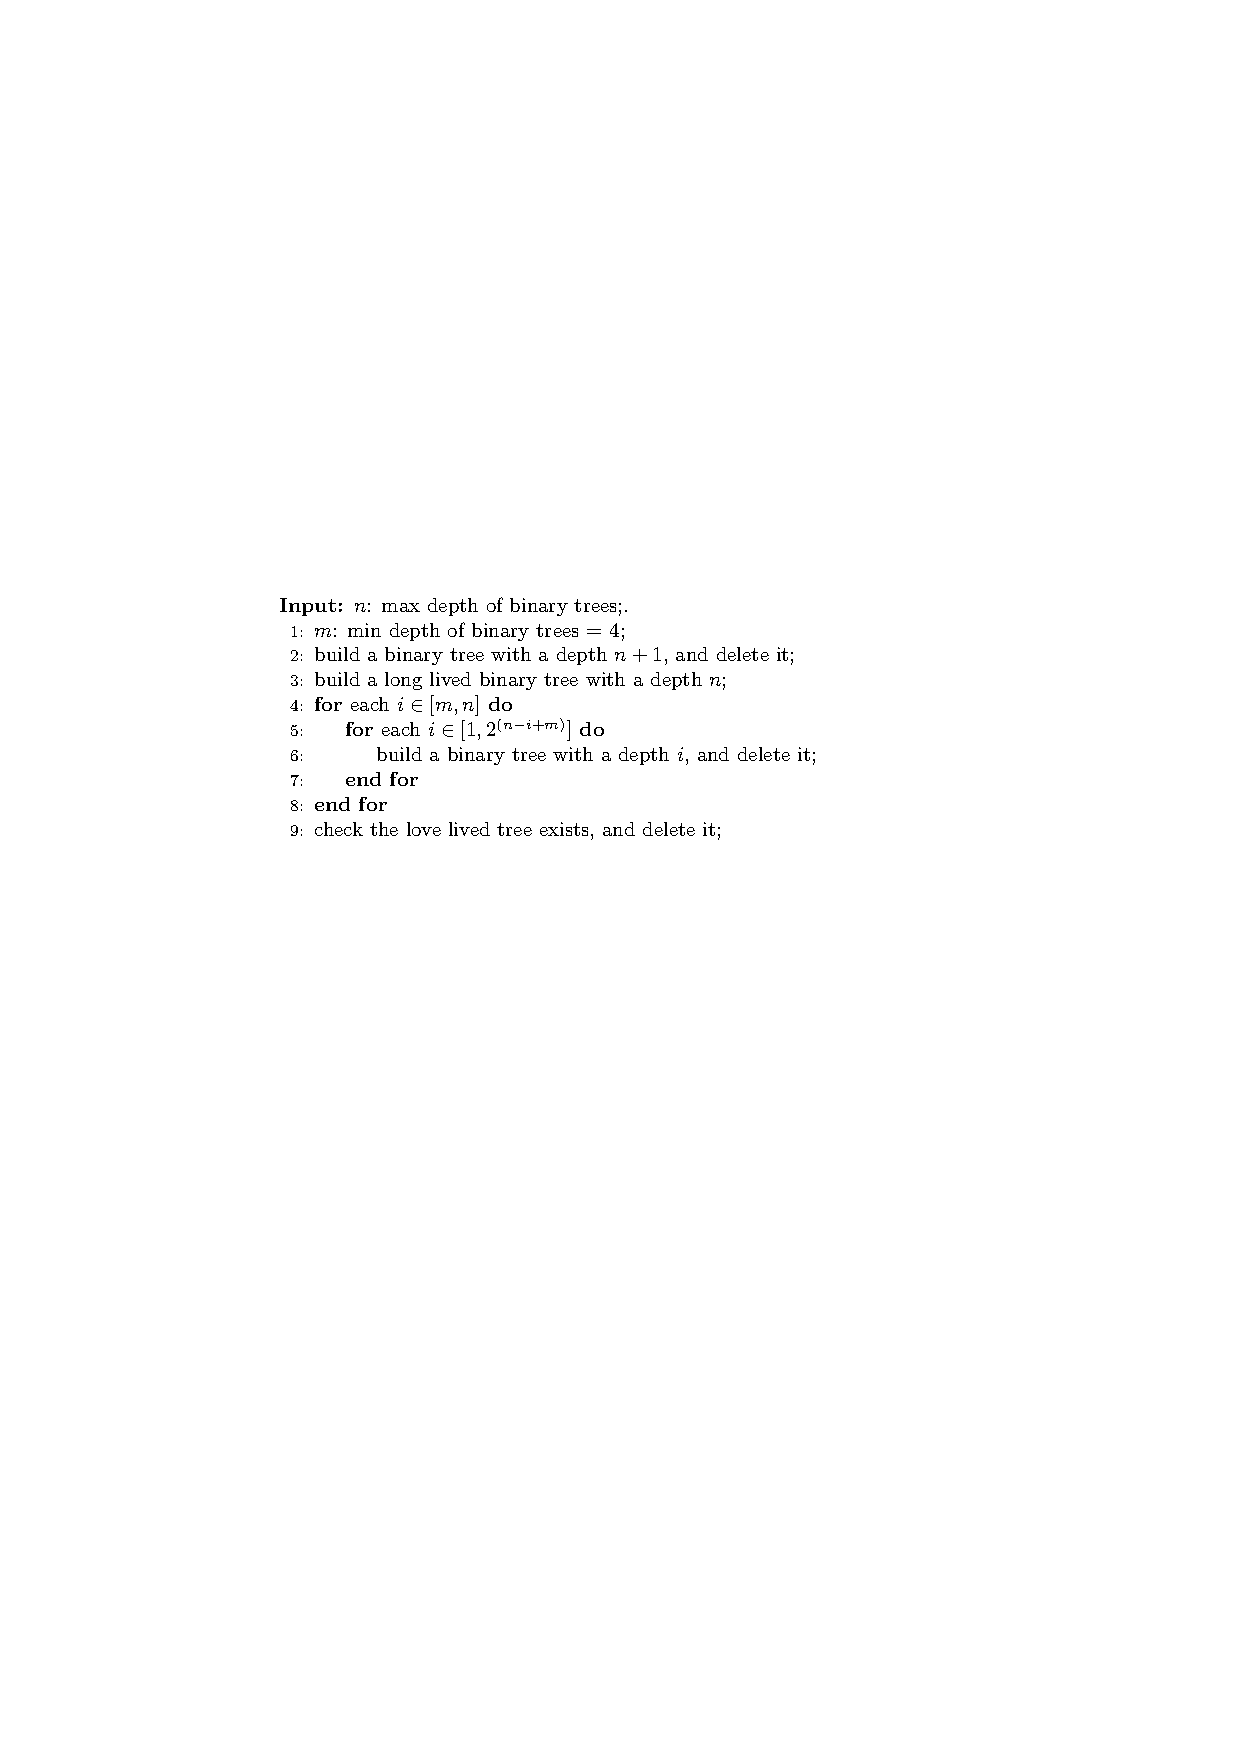
\includegraphics[scale=0.8]{figures/mandelbrot}}
    \label{fig:mandelbrot}
\end{figure}

\begin{table}[ht]
    \caption{Comprehensive test - large input}
    \label{tab:mandelbrot-1}
    \begin{center}
        \begin{tabular}{lrrrr}
            \toprule
            lang      & n     & size(B) & cpu(s)  & mem(KB) \\
            \midrule
            cpp-clang & 16000 & 822     & 13.900  & 30172   \\
            cpp-gcc   & 16000 & 822     & 13.931  & 28696   \\
            dart-aot  & 16000 & 454     & 154.089 & 17240   \\
            dart-jit  & 16000 & 454     & 151.501 & 148144  \\
            go        & 16000 & 823     & 19.598  & 32412   \\
            java      & 16000 & 665     & 27.834  & 34264   \\
            js-node   & 16000 & 373     & 130.638 & 42020   \\
            kt-jvm    & 16000 & 407     & 30.032  & 28432   \\
            python3   & 16000 & 688     & 702.599 & 47780   \\
            rust      & 16000 & 868     & 11.904  & 38528   \\
            swift     & 16000 & 394     & 26.277  & 6200    \\
            \bottomrule
        \end{tabular}
    \end{center}
\end{table}


\begin{table}[htbp]
    \caption{Comprehensive test - small input}
    \label{tab:mandelbrot-2}
    \begin{center}
        \begin{tabular}{lrrrr}
            \toprule
            lang      & n    & size(B) & cpu(s) & mem(KB) \\
            \midrule
            cpp-clang & 4000 & 822     & 0.880  & 1552    \\
            cpp-gcc   & 4000 & 822     & 0.881  & 1192    \\
            dart-aot  & 4000 & 454     & 10.276 & 17380   \\
            dart-jit  & 4000 & 454     & 10.096 & 148084  \\
            go        & 4000 & 823     & 1.260  & 2420    \\
            java      & 4000 & 665     & 1.827  & 34352   \\
            js-node   & 4000 & 373     & 8.763  & 42540   \\
            kt-jvm    & 4000 & 407     & 2.419  & 28448   \\
            python3   & 4000 & 688     & 46.273 & 12172   \\
            rust      & 4000 & 868     & 0.757  & 4388    \\
            swift     & 4000 & 394     & 1.661  & 6240    \\
            \bottomrule
        \end{tabular}
    \end{center}
\end{table}

For the same Dart code, it is compiled in two different ways,
using JIT and AOT. As for the time and memory overhead in Table~\ref{tab:mandelbrot-1} and Table~\ref{tab:mandelbrot-2},
both have similar performance. This is caused by the compilation mechanism of Dart. In fact, the running mechanism of Dart is different from the traditional way. The traditional AOT is to compile the source code directly into the object code on the target machine, which can be called and run independently by the operating system directly. However, for Dart, whether it is AOT or JIT, only the compilation time is different, and it will eventually run on the virtual machine. In fact, when the compilation time is negligible, the time overhead of AOT and JIT is approximately equal. But this way of running has its unique disadvantage. It will significantly increase the running overhead of AOT mode, but this makes AOT compilation has strong runtime support. Because of this feature, the Dart VM can save the current runtime state, and the next time the VM is started, it can directly load the last state without restarting. This is mainly for a better development experience. The incremental compilation feature allows the runtime results to change almost in real time as the code is changed. Dart is a language for the front-end cross-platform framework Flutter. With such a mechanism, code changes can feed back to the UI in real-time, which is hard to do with other languages.

In industrial applications, the performance bottleneck in most scenarios is compile-related, including not only compile-time but also run-time. The impact of compilation on programming language efficiency is again multifaceted. First, the same programming language with different compilers will often have different object code and thus different runtime efficiency. This is often due to different compile-time optimizations; for example, for C++, there is a significant performance difference in the object code obtained by compiling with Clang-LLVM as opposed to compiling with GCC. Second, the same programming language can run not only in AOT, but also in JIT. For example, for Kotlin, it can be compiled not only as bytecode to run on JVM, but also programmed as JavaScript code to run on the browser, or even Kotlin Native, which can run as native code. In this way, the different compilation methods have a greater impact on efficiency.

The impact of memory management on programming language performance is huge. First, there is the matter of memory allocation on the heap. For languages with VM, memory allocation is an advantage compared to non-VM languages. This is because VM languages provide memory pools that host the memory allocation, whereas non-VM languages do not have such an advantage. Of course, for scenarios where memory on the heap is used frequently, non-VM languages tend to use custom or third-party provided memory pooling frameworks, and the performance gap in the industry is not as pronounced. But managed memory is not always an advantage. When a memory thrash occurs, the VM will frequently GC, which also affects performance. And, memory pools tend to have a larger memory overhead. Second, there is the principle of locality about memory. CPU will put all the adjacent data into cache, and if the memory is accessed sequentially, it greatly improves the hit rate of cache, thus improving the performance.

    \section{Conclusion}

%Currently, the analysis of programming language design is still relatively rare compared to the mainstream research direction of PLT. In particular, a systematic approach to the study of programming language design is still lacking. In this paper, we present a relatively comprehensive analysis of programming language design through several aspects affecting programming language applications with the help of several specific MPLs.
%
%In Chapter 2, we discuss the definition of MPL. Based on that, the popular programming languages on IEEE Spectrum with MPL features are selected. Then we discuss the factors that a good programming language design should have. In Chapter 3, we stand in the perspective of programming paradigms, give a method to judge the degree of MPL programming paradigm support, and do an analysis of the degree of support of the selected MPLs. This is followed by an research of the relationship between the strength of programming paradigm support and programming language applications. In Chapter 4, we discuss the type system. The type system of the selected MPLs is discussed based on L Cardelli's type system definition. In Chapter 5, we discuss the performance of programming languages through three benchmark tests in terms of memory allocation and compilation methods. Then, we analyze the data from the benchmark tests from the perspective of programming language implementations and the application scenarios of these languages to explain the reasons for the performance of these MPLs.
%
%Programming paradigms, type systems, and performance are three interconnected parts that cut across multiple aspects of programming languages that need to be considered from design to implementation. Each of these three branches has a significant impact on the design of programming languages, influencing their expressiveness, maintainability, reliability, and performance, the most important metrics of programming languages. In fact we can obtain that the process of theoretical and practical development of programming languages is always dynamic, as is the design and implementation of programming languages. Programming paradigms, type systems, and performance are three interconnected parts that cut across multiple aspects of programming languages that need to be considered from design to implementation. Each of these three branches has a significant impact on the design of programming languages, influencing their expressiveness, maintainability, reliability, and performance, the most important metrics of programming languages. In fact we can obtain that the process of theoretical and practical development of programming languages is always dynamic, as is the design and implementation of programming languages. This paper dynamically discusses programming language design based on MPL, which would be a preferable research idea from a programming language design and analysis perspective.


Currently, the research on programming language design is still relatively rare compared to the mainstream research direction of PLT which is the implementation of programming language. In this paper, we present a relatively comprehensive analysis of the design of multiple MPLs through several aspects affecting their applications.

We first select some popular programming languages on IEEE Spectrum with MPL features after discussing the definition of MPL. Then we discuss the features that a well-designed programming language should have. Next, we stand in the perspective of programming paradigms to give a method to judge the degree of MPLs’ paradigm support, and do an analysis of the selected MPL, followed by the relationship between the degree of programming paradigm support and programming language applications. Furthermore, the type systems of the selected MPLs are discussed based on L. Cardelli’s definition of type systems. Finally, we evaluate the performance of the selected MPLs through three benchmark tests and explain the reasons for the performance from the perspective of programming language implementations and their application scenarios.

Programming paradigms, type systems, and performance are three critical interconnected parts that have a significant impact on the design of programming languages, influencing their most important metrics, namely expressiveness, maintainability, reliability, and performance. In fact, the theory and practice of programming languages are always dynamically developing, as are their design and implementation. This paper comprehensively discusses the design of certain MPLs, which would be a practical reference and a valuable inspiration for programming language developers and programmers.



    \bibliographystyle{IEEEtran}
    \bibliography{IEEEabrv,main}
\end{document}
